\documentclass[11pt]{article}            % Report class in 11 points
\parindent0pt  \parskip10pt             % make block paragraphs
\usepackage{graphicx}
\usepackage{listings}
\graphicspath{ {images/} }
\usepackage{graphicx} %  graphics header file
\begin{document}
\begin{titlepage}
    \centering
  \vfill
    
\includegraphics[width=8cm]{uni_logo.png} \\ 
	\vskip2cm
    {\bfseries\Large
	Artificial Intelligence \\ (CS13217)\\
	
	\vskip2cm
	Lab Report 
	 
	\vskip2cm
	}    

\begin{center}
\begin{tabular}{ l l  } 

Name: & Kanza Afzal \\ 
Registration \#: & CSU-XS18-132 \\ 
Lab Report \#: & 01 \\ 
 Dated:& 16-03-2018\\ 
Submitted To:& Mr. Usman Ahmed\\ 

 %\hline
\end{tabular}
\end{center}
    \vfill
    The University of Lahore, Islamabad Campus\\
Department of Computer Science \& Information Technology
\end{titlepage}


    
    {\bfseries\Large
\centering
	Experiment \# 1 \\

Installationthe setup of Python\\
	
	}    
 \vskip1cm
 \textbf {Objective}\\  To download and install the setup of  Python
 
 \textbf {Software Tool} \\
1. Operating system window 10 \\
2.  sublime version 3.0\\
3.  python\\

\subsection{Procedure: Task 1 }     
\section{Python downloading Steps }  
      

   
1.The following screen will be show on google chrome.\\

\begin{center}
  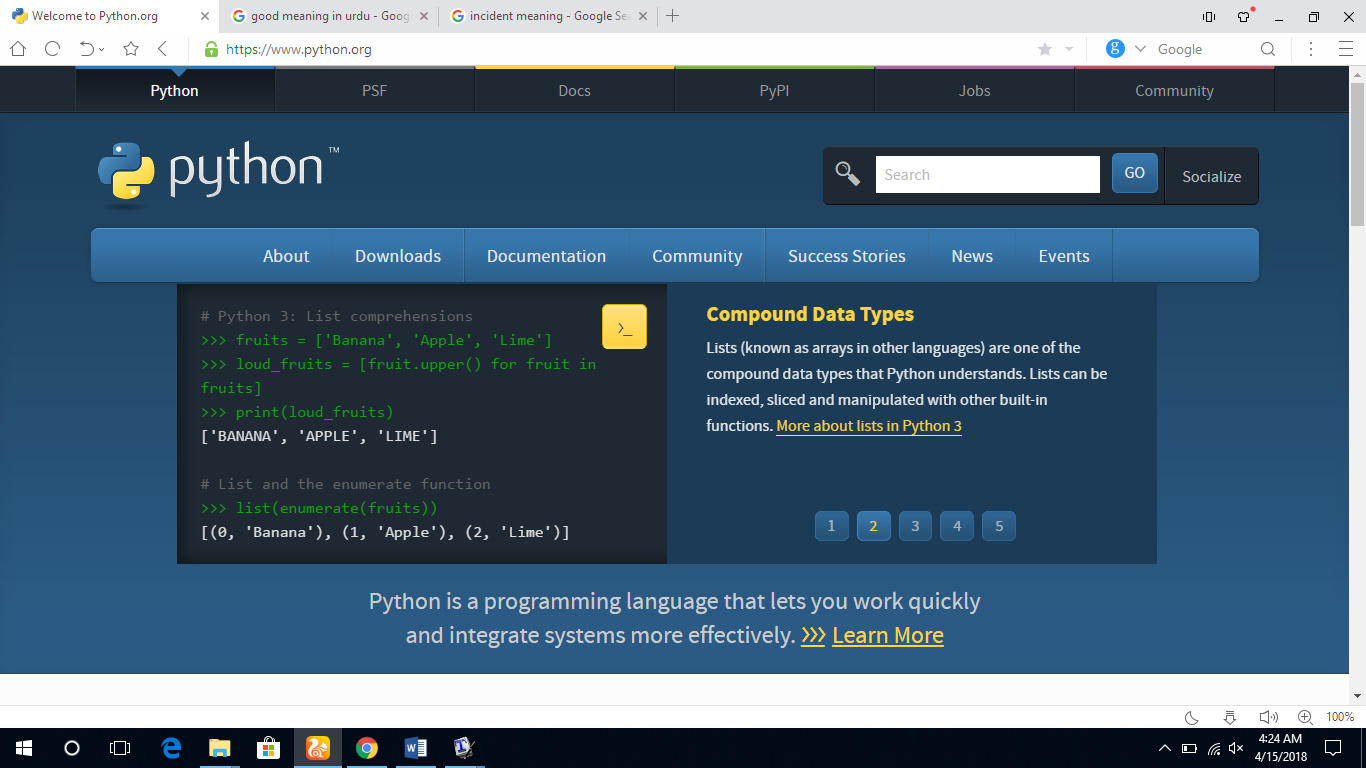
\includegraphics[width=12cm,height=6cm,keepaspectratio]{9.png}\\
\end{center}

2. Click the download Python 2.7.13\\ 
3. The file named python-2.7.13exe should start downloading into your standard download folder. \\
4. Move this file to a more permanent location, so that you can install Python.\\
5. Feel free to explore this webpage further; if you want to just continue the installation, you can terminate the tab browsing this webpage.\\
6. Start the Installing instructions directly given below .\\

\begin{center}
  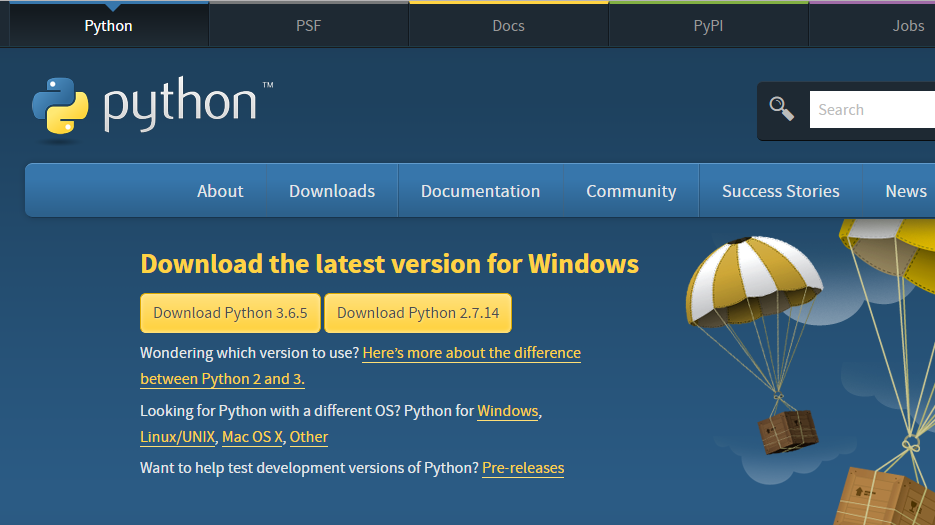
\includegraphics[width=12cm,height=6cm,keepaspectratio]{1.png}\\
\end{center}


\section{Procedure: Task 2 }   
  
\subsection{Python Installations Steps }  

1. Double-click the icon labeling the file python-2.7.14 exe.\\


\begin{center}
  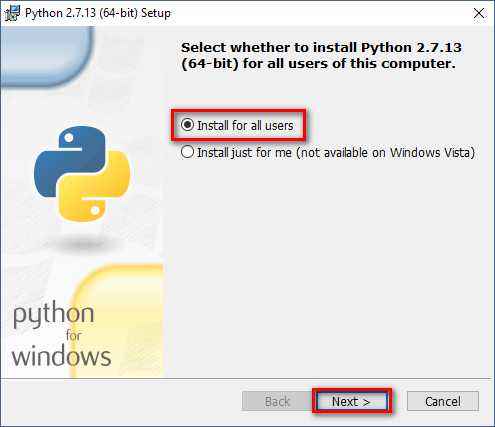
\includegraphics[width=12cm,height=6cm,keepaspectratio]{2.png}\\ 

\end{center} 
.


2. Select the destination directory\\ 


\begin{center}
  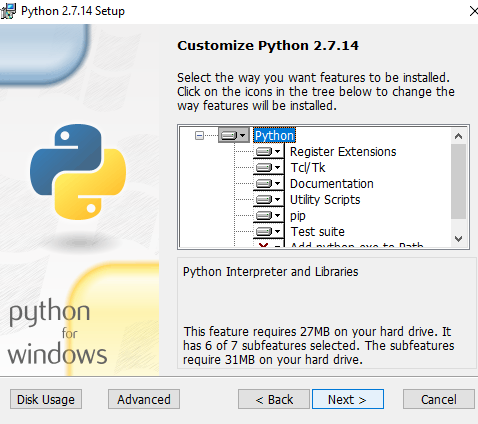
\includegraphics[width=12cm,height=6cm,keepaspectratio]{5.png}\\
\end{center}

Ensure that the Install launcher for all users (recommended) and the Add \\ Python 2.6 to PATH checkboxes at the bottom are checked

3. Click the Yes button.\\

\begin{center}
  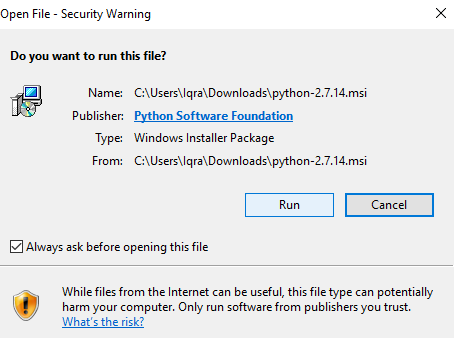
\includegraphics[width=12cm,height=6cm,keepaspectratio]{8.png}\\
\end{center}


4.  A new Python 2.7.13 (64-bit) Setup pop-up window will appear with a Setup Progress message and a progress bar.\\
  



5.  During installation, it will show the various components it is installing and move the progress bar towards completion.
   Soon, a new Python 2.7.13 (64-bit) Setup pop-up window will appear with a Setup was successfuly message.\\ 

\begin{center}
  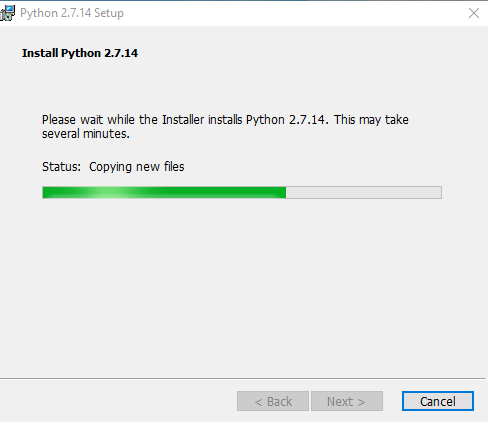
\includegraphics[width=12cm,height=6cm,keepaspectratio]{6.png}\\
\end{center}



5. Click the Finish button.\\ 
\begin{center}

  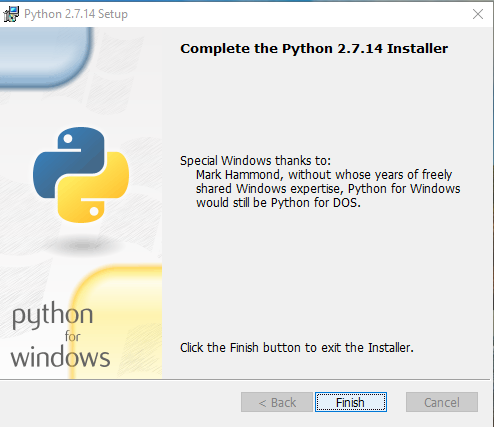
\includegraphics[width=12cm,height=6cm,keepaspectratio]{4.png}\\
\end{center}






\section{Conclusion}  
Successfullly the setup of Python woulid be downloaded and installed.
 
\end{document}                          % The required last line
